\chapter{Resultados processamento de imagem }

Características da máquina de processamento  
\begin{itemize}
	\item CPU: Intel Core i7-3630QM CPU @ 2.40GHz x 8
	\item SO version: Ubuntu 16.04.2 LTS
	\item Intel Corporation 3rd Gen Core processor Graphics Controller (rev 09)
	NVIDIA Corporation GF108M [GeForce GT 635M] (rev a1)
\end{itemize}

%Intel® Core™ i7-3630QM CPU @ 2.40GHz × 8
Todas as frames apresentadas de seguida apresentam as seguintes caracteristicas: 
\begin{itemize}
	\item Dimensões (px): 1366 x 768
	\item Tamanho (MB): 1.2 
\end{itemize}


\section{Frame 1}

\begin{figure}[!htb]
	\centering
	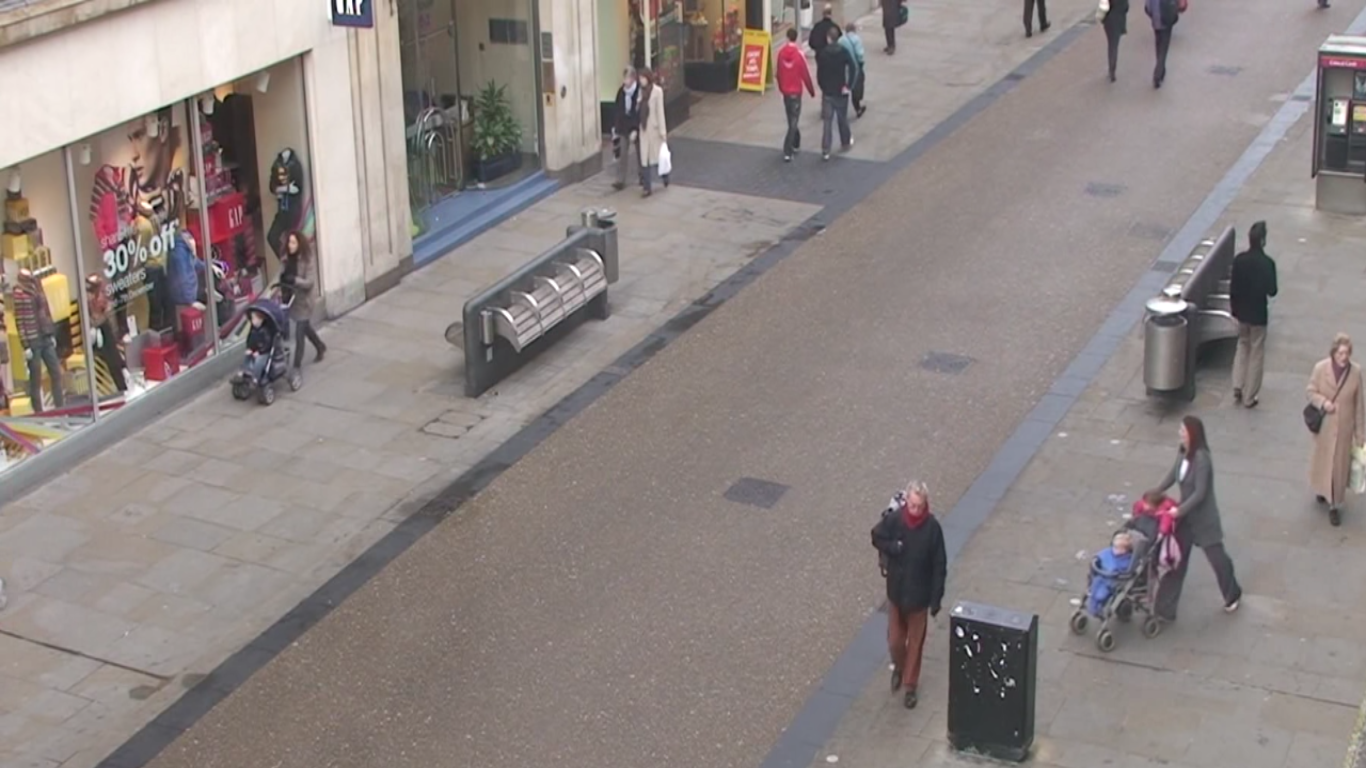
\includegraphics[width=0.5\linewidth]{img/vision/frame1.png}
	\caption{Frame 1 }
	\label{db}
\end{figure}

\textbf{Número de pessoas existentes neste frame}: 9

\begin{longtable}{|l|l|l|l|l|l|} 
	\hline
	\textbf{winStride} & \textbf{padding} & \textbf{scale} & \textbf{detection (number)} & \textbf{execution time (seg)} \\ \hline
	(2, 2) & (8, 8) & 0.5 & 7 & 1.26149988174 \\ \hline
	(4, 4) & (8, 8) & 0.5 & 2 & 0.375313043594 \\ \hline
	(8, 8) & (8, 8) & 0.5 & 0 & 0.135497093201 \\ \hline
	(2, 2) & (8, 8) & 1.0 & 7 & 1.3139770031 \\ \hline
	(4, 4) & (8, 8) & 1.0 & 2 & 0.372344970703 \\ \hline
	(8, 8) & (8, 8) & 1.0 & 0 & 0.132822036743 \\ \hline
	(2, 2) & (8, 8) & 1.5 & 12 & 1.32045602798 \\ \hline
	(4, 4) & (8, 8) & 1.5 & 6 & 0.371366977692 \\ \hline
	(8, 8) & (8, 8) & 1.5 & 0 & 0.167386054993 \\ \hline
	(2, 2) & (16, 16) & 0.5 & 8 & 1.3565030098 \\ \hline
	(4, 4) & (16, 16) & 0.5 & 2 & 0.383218050003 \\ \hline
	(8, 8) & (16, 16) & 0.5 & 0 & 0.132525205612 \\ \hline
	(2, 2) & (16, 16) & 1.0 & 8 & 1.33558607101 \\ \hline
	(4, 4) & (16, 16) & 1.0 & 2 & 0.362588882446 \\ \hline
	(8, 8) & (16, 16) & 1.0 & 0 & 0.131352186203 \\ \hline
	(2, 2) & (16, 16) & 1.5 & 13 & 1.2949719429 \\ \hline
	(4, 4) & (16, 16) & 1.5 & 6 & 0.434331178665 \\ \hline
	(8, 8) & (16, 16) & 1.5 & 0 & 0.1577501297 \\ \hline
	(2, 2) & (24, 24) & 0.5 & 8 & 1.37960910797 \\ \hline
	(4, 4) & (24, 24) & 0.5 & 2 & 0.374704837799 \\ \hline
	(8, 8) & (24, 24) & 0.5 & 0 & 0.136407852173 \\ \hline
	(2, 2) & (24, 24) & 1.0 & 8 & 1.33125019073 \\ \hline
	(4, 4) & (24, 24) & 1.0 & 2 & 0.372330904007 \\ \hline
	(8, 8) & (24, 24) & 1.0 & 0 & 0.132616996765 \\ \hline
	(2, 2) & (24, 24) & 1.5 & 13 & 1.36268496513 \\ \hline
	(4, 4) & (24, 24) & 1.5 & 7 & 0.421048164368 \\ \hline
	(8, 8) & (24, 24) & 1.5 & 0 & 0.183830022812 \\ \hline

		
	\caption{Your caption here} % needs to go inside longtable environment
	\label{tab:myfirstlongtable}
\end{longtable}


\newpage
\section{Frame 2}

\begin{figure}[h]
	\centering
	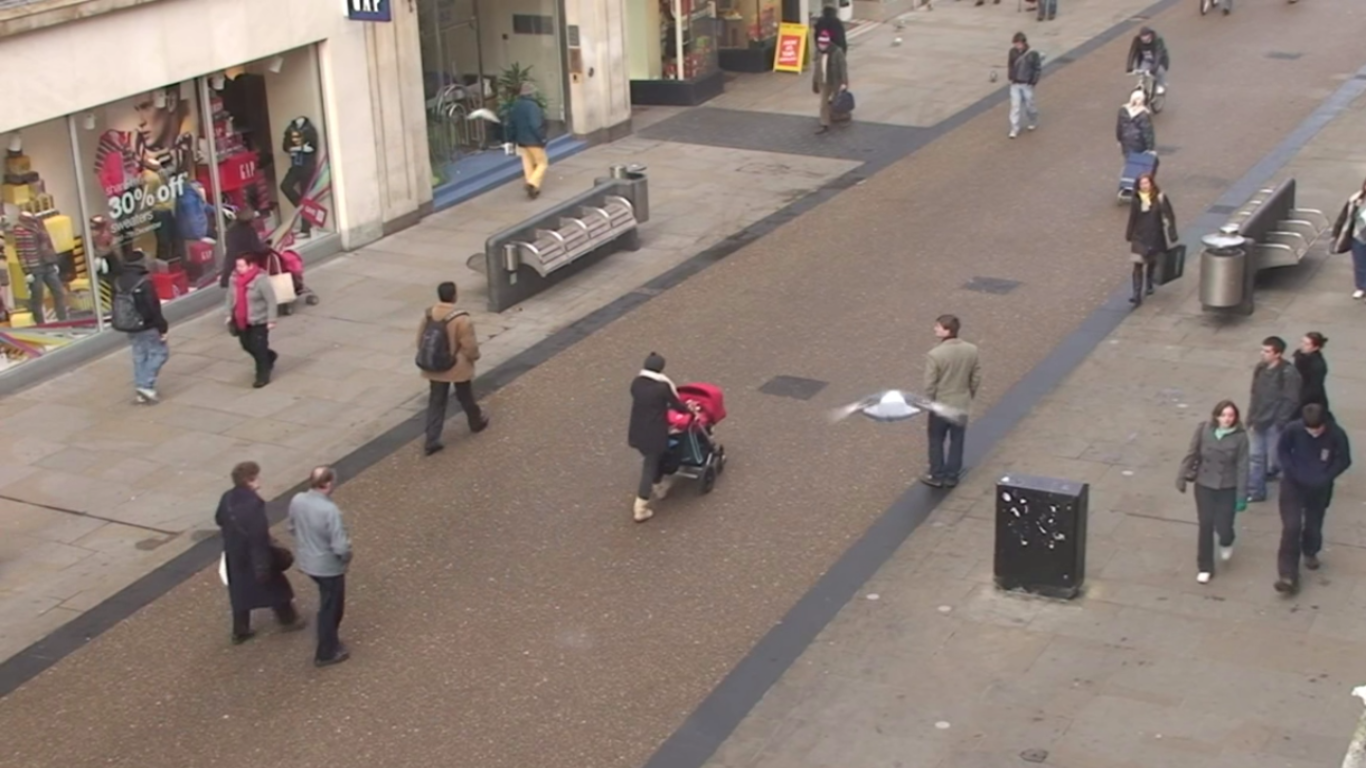
\includegraphics[width=0.5\linewidth]{img/vision/frame2.png}
	\caption{Frame 2 }
	\label{db}
\end{figure}

\textbf{Número de pessoas existentes neste frame}: 14


\begin{longtable}{|l|l|l|l|l|l|} 
	\hline
	\textbf{winStride} & \textbf{padding} & \textbf{scale} & \textbf{detection (number)} & \textbf{execution time (seg)} \\ \hline
	(2, 2) & (8, 8) & 0.5 & 5 & 1.26896286011 \\ \hline
	(4, 4) & (8, 8) & 0.5 & 2 & 0.355625867844 \\ \hline
	(8, 8) & (8, 8) & 0.5 & 0 & 0.132093906403 \\ \hline
	(2, 2) & (8, 8) & 1.0 & 5 & 1.27296304703 \\ \hline
	(4, 4) & (8, 8) & 1.0 & 2 & 0.357967853546 \\ \hline
	(8, 8) & (8, 8) & 1.0 & 0 & 0.131447076797 \\ \hline
	(2, 2) & (8, 8) & 1.5 & 10 & 1.31779408455 \\ \hline
	(4, 4) & (8, 8) & 1.5 & 7 & 0.381912946701 \\ \hline
	(8, 8) & (8, 8) & 1.5 & 2 & 0.162096977234 \\ \hline
	(2, 2) & (16, 16) & 0.5 & 5 & 1.29711699486 \\ \hline
	(4, 4) & (16, 16) & 0.5 & 2 & 0.360393047333 \\ \hline
	(8, 8) & (16, 16) & 0.5 & 0 & 0.130337953568 \\ \hline
	(2, 2) & (16, 16) & 1.0 & 5 & 1.29114198685 \\ \hline
	(4, 4) & (16, 16) & 1.0 & 2 & 0.365696191788 \\ \hline
	(8, 8) & (16, 16) & 1.0 & 0 & 0.130436897278 \\ \hline
	(2, 2) & (16, 16) & 1.5 & 11 & 1.30830812454 \\ \hline
	(4, 4) & (16, 16) & 1.5 & 7 & 0.472708940506 \\ \hline
	(8, 8) & (16, 16) & 1.5 & 2 & 0.213890075684 \\ \hline
	(2, 2) & (24, 24) & 0.5 & 5 & 1.493486166 \\ \hline
	(4, 4) & (24, 24) & 0.5 & 2 & 0.385469913483 \\ \hline
	(8, 8) & (24, 24) & 0.5 & 0 & 0.134639978409 \\ \hline
	(2, 2) & (24, 24) & 1.0 & 5 & 1.32583999634 \\ \hline
	(4, 4) & (24, 24) & 1.0 & 2 & 0.373645067215 \\ \hline
	(8, 8) & (24, 24) & 1.0 & 0 & 0.133275985718 \\ \hline
	(2, 2) & (24, 24) & 1.5 & 11 & 1.35700201988 \\ \hline
	(4, 4) & (24, 24) & 1.5 & 8 & 0.461907863617 \\ \hline
	(8, 8) & (24, 24) & 1.5 & 2 & 0.157855033875 \\ \hline
	
	\caption{Your caption here} % needs to go inside longtable environment
	\label{tab:myfirstlongtable}
\end{longtable}



\section{Frame 3}


\begin{figure}[h]
	\centering
	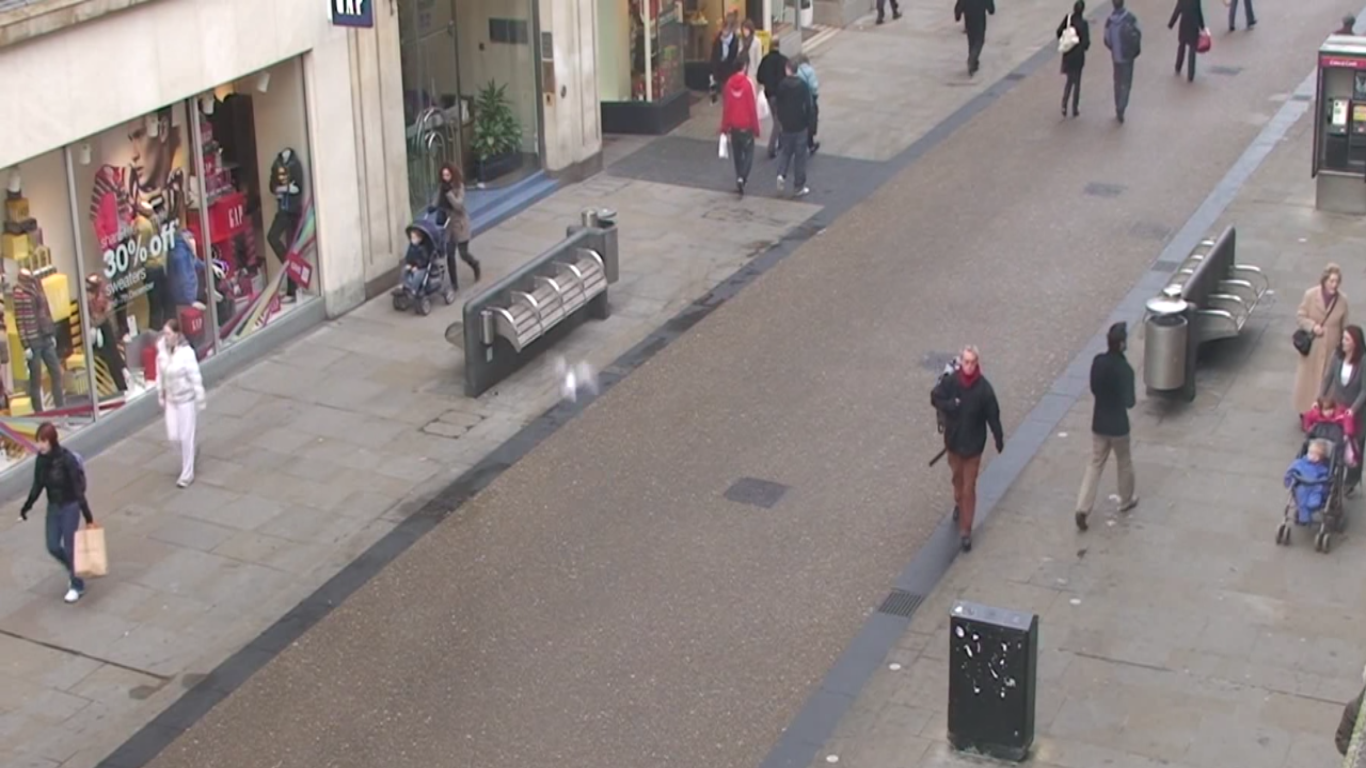
\includegraphics[width=0.7\linewidth]{img/vision/frame3.png}
	\caption{Frame 3 }
	\label{db}
\end{figure}

\textbf{Número de pessoas existentes neste frame}: 12


\begin{longtable}{|l|l|l|l|l|l|} 
	\hline
	\textbf{winStride} & \textbf{padding} & \textbf{scale} & \textbf{detection (number)} & \textbf{execution time (seg)} \\ \hline
(2, 2) & (8, 8) & 0.5 & 9 & 1.27664995193 \\ \hline
(4, 4) & (8, 8) & 0.5 & 4 & 0.358872890472 \\ \hline
(8, 8) & (8, 8) & 0.5 & 0 & 0.12829208374 \\ \hline
(2, 2) & (8, 8) & 1.0 & 9 & 1.24722003937 \\ \hline
(4, 4) & (8, 8) & 1.0 & 4 & 0.359780788422 \\ \hline
(8, 8) & (8, 8) & 1.0 & 0 & 0.134448051453 \\ \hline
(2, 2) & (8, 8) & 1.5 & 12 & 1.33601593971 \\ \hline
(4, 4) & (8, 8) & 1.5 & 8 & 0.369907855988 \\ \hline
(8, 8) & (8, 8) & 1.5 & 0 & 0.204400062561 \\ \hline
(2, 2) & (16, 16) & 0.5 & 9 & 1.35411095619 \\ \hline
(4, 4) & (16, 16) & 0.5 & 4 & 0.369040966034 \\ \hline
(8, 8) & (16, 16) & 0.5 & 0 & 0.136008024216 \\ \hline
(2, 2) & (16, 16) & 1.0 & 9 & 1.3030230999 \\ \hline
(4, 4) & (16, 16) & 1.0 & 4 & 0.38528585434 \\ \hline
(8, 8) & (16, 16) & 1.0 & 0 & 0.137537956238 \\ \hline
(2, 2) & (16, 16) & 1.5 & 11 & 1.37075090408 \\ \hline
(4, 4) & (16, 16) & 1.5 & 9 & 0.369807004929 \\ \hline
(8, 8) & (16, 16) & 1.5 & 0 & 0.172605991364 \\ \hline
(2, 2) & (24, 24) & 0.5 & 10 & 1.32573390007 \\ \hline
(4, 4) & (24, 24) & 0.5 & 5 & 0.374289989471 \\ \hline
(8, 8) & (24, 24) & 0.5 & 0 & 0.135723114014 \\ \hline
(2, 2) & (24, 24) & 1.0 & 10 & 1.37439012527 \\ \hline
(4, 4) & (24, 24) & 1.0 & 5 & 0.377769947052 \\ \hline
(8, 8) & (24, 24) & 1.0 & 0 & 0.134618997574 \\ \hline
(2, 2) & (24, 24) & 1.5 & 12 & 1.35487890244 \\ \hline
(4, 4) & (24, 24) & 1.5 & 10 & 0.408782958984 \\ \hline
(8, 8) & (24, 24) & 1.5 & 0 & 0.147122144699 \\ \hline


	\caption{Your caption here} % needs to go inside longtable environment
	\label{tab:myfirstlongtable}
\end{longtable}

\section{Frame 4}

\begin{figure}[h]
	\centering
	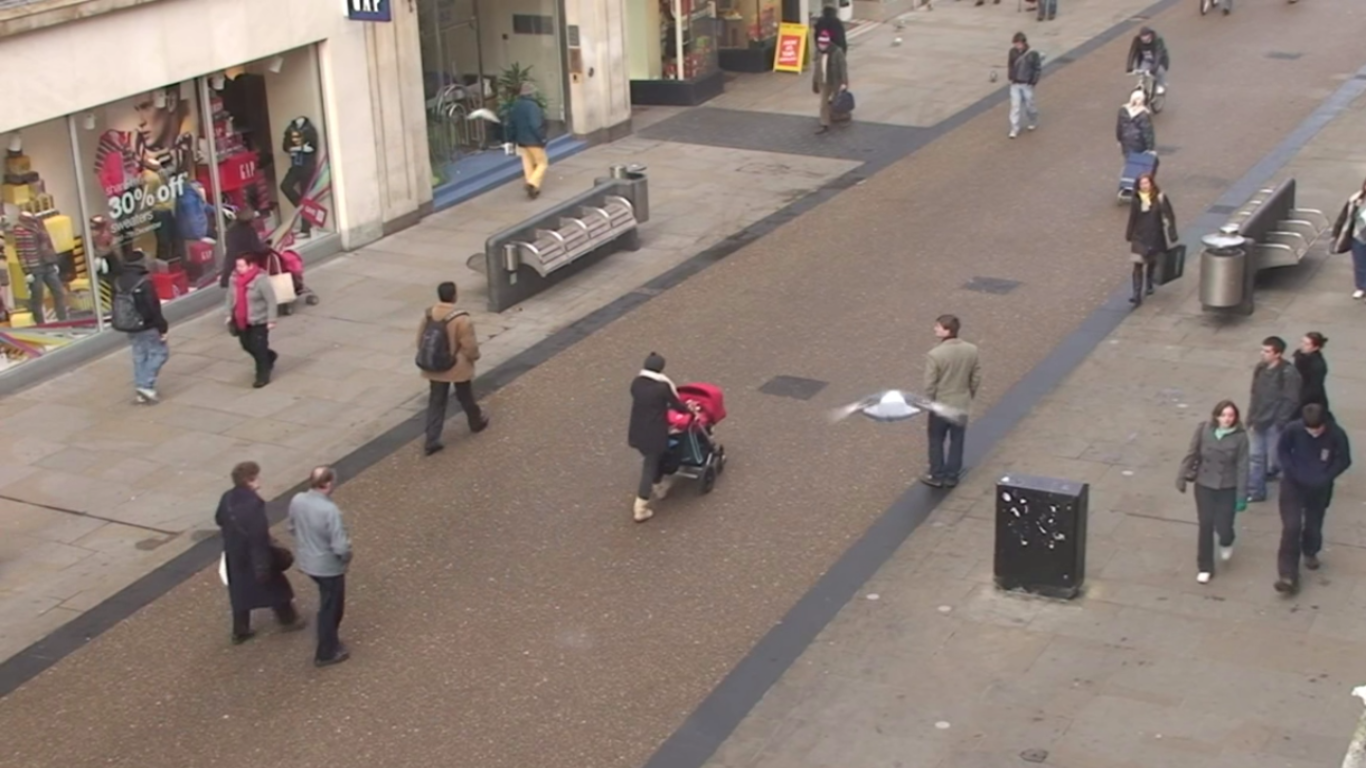
\includegraphics[width=0.5\linewidth]{img/vision/frame4.png}
	\caption{Frame 3 }
	\label{db}
\end{figure}

\textbf{Número de pessoas existentes neste frame}: 6

\begin{longtable}{|l|l|l|l|l|l|} 
	\hline
	\textbf{winStride} & \textbf{padding} & \textbf{scale} & \textbf{detection (number)} & \textbf{execution time (seg)} \\ \hline
(2, 2) & (8, 8) & 0.5 & 3 & 1.34746980667 \\ \hline
(4, 4) & (8, 8) & 0.5 & 1 & 0.363748073578 \\ \hline
(8, 8) & (8, 8) & 0.5 & 0 & 0.132915019989 \\ \hline
(2, 2) & (8, 8) & 1.0 & 3 & 1.27492785454 \\ \hline
(4, 4) & (8, 8) & 1.0 & 1 & 0.357720851898 \\ \hline
(8, 8) & (8, 8) & 1.0 & 0 & 0.130718946457 \\ \hline
(2, 2) & (8, 8) & 1.5 & 8 & 1.42473483086 \\ \hline
(4, 4) & (8, 8) & 1.5 & 4 & 0.393920898438 \\ \hline
(8, 8) & (8, 8) & 1.5 & 1 & 0.131416082382 \\ \hline
(2, 2) & (16, 16) & 0.5 & 3 & 1.35367703438 \\ \hline
(4, 4) & (16, 16) & 0.5 & 2 & 0.365742921829 \\ \hline
(8, 8) & (16, 16) & 0.5 & 0 & 0.133272886276 \\ \hline
(2, 2) & (16, 16) & 1.0 & 3 & 1.2900660038 \\ \hline
(4, 4) & (16, 16) & 1.0 & 2 & 0.360087156296 \\ \hline
(8, 8) & (16, 16) & 1.0 & 0 & 0.131268024445 \\ \hline
(2, 2) & (16, 16) & 1.5 & 8 & 1.36765789986 \\ \hline
(4, 4) & (16, 16) & 1.5 & 5 & 0.481853961945 \\ \hline
(8, 8) & (16, 16) & 1.5 & 1 & 0.176377058029 \\ \hline
(2, 2) & (24, 24) & 0.5 & 3 & 1.40264105797 \\ \hline
(4, 4) & (24, 24) & 0.5 & 2 & 0.392567873001 \\ \hline
(8, 8) & (24, 24) & 0.5 & 0 & 0.137512922287 \\ \hline
(2, 2) & (24, 24) & 1.0 & 3 & 1.35502314568 \\ \hline
(4, 4) & (24, 24) & 1.0 & 2 & 0.380364894867 \\ \hline
(8, 8) & (24, 24) & 1.0 & 0 & 0.136371135712 \\ \hline
(2, 2) & (24, 24) & 1.5 & 9 & 1.65068483353 \\ \hline
(4, 4) & (24, 24) & 1.5 & 5 & 0.401294946671 \\ \hline
(8, 8) & (24, 24) & 1.5 & 1 & 0.206337928772 \\ \hline

	
	\caption{Your caption here} % needs to go inside longtable environment
	\label{tab:myfirstlongtable}
\end{longtable}
